\documentclass{article}

\usepackage{amsmath}
\usepackage{amssymb}
\usepackage{mathpartir}
\usepackage{fontawesome5}
\usepackage{xcolor}
\usepackage{tikz}
\mprset{flushleft}
\newcommand{\kw}[1]{\text{\textbf{#1}}}
\newcommand{\Let}[3]{\kw{let}\, #1 = #2\, \kw{in}\, #3}
\newcommand{\Fun}[2]{\kw{fun}\, #1 \Rightarrow #2}
\newcommand{\App}[2]{#1\, #2}
\newcommand{\Pair}[2]{(#1, #2)}
\newcommand{\LetPair}[4]{\kw{let}\, (#1, #2) = #3\, \kw{in}\, #4}
\newcommand{\Inl}[1]{\kw{left}(#1)}
\newcommand{\Inr}[1]{\kw{right}(#1)}
\newcommand{\Match}[5]{\kw{match}\, #1\, \kw{with}\, \Inl{#2} \Rightarrow #3 \mid \Inr{#4} \Rightarrow #5}
\newcommand{\AnnotSub}[1]{%
  \if\relax\detokenize{#1}\relax
  \else
    _{\smash{\raisebox{-0.25ex}{$\scriptstyle #1$}}}
  \fi}
\newcommand{\RefCell}[1]{\kw{ref}\, #1}
\newcommand{\Deref}[1]{\ !#1}
\newcommand{\Assign}[2]{#1 := #2}
\newcommand{\AnnotArrow}[1]{%
  \if\relax\detokenize{#1}\relax
    \to
  \else
    \xrightarrow[\AnnotBelow{#1}]{}
  \fi}
\newcommand{\AnnotBinop}[2]{%
  \if\relax\detokenize{#2}\relax
    #1
  \else
    \underset{\AnnotBelow{#2}}{#1}
  \fi}
\newcommand{\AnnotBelow}[1]{\smash{\raisebox{0.25ex}{$\scriptstyle #1$}}}
\newcommand{\TFun}[3][]{#2 \mathrel{\AnnotArrow{#1}} #3}
\newcommand{\TPair}[3][]{#2 \mathbin{\AnnotBinop{\times}{#1}} #3}
\newcommand{\TSum}[3][]{#2 \mathbin{\AnnotBinop{+}{#1}} #3}
\newcommand{\TRef}[2][]{\kw{ref}\AnnotSub{#1}\, #2}
\newcommand{\TUnit}{\kw{unit}}
\newcommand{\TEmpty}{\kw{empty}}
\newcommand{\UnitTerm}{\kw{unit}}
\newcommand{\Absurd}[1]{\kw{absurd}\, #1}
\newcommand{\judge}[3]{#1 \vdash #2 : #3}
\newcommand{\Jud}[2]{\judge{\Gamma}{#1}{#2}}
\newcommand{\leqto}{\mathrel{\leq_{\mathrm{to}}}}
\newcommand{\leqin}{\mathrel{\leq_{\mathrm{in}}}}
\newcommand{\mode}[1]{\textsc{#1}}
\newcommand{\subtype}{\mathrel{\sqsubseteq}}
\newcommand{\Sub}[2]{#1 \subtype #2}
\newcommand{\alias}{\mathrel{\underset{\AnnotBelow{\text{alias}}}{\rightsquigarrow}}}
\newcommand{\Alias}[2]{#1 \alias #2}
\newcommand{\Lock}[2][]{
  \text{\faLock}_{#1}(#2)
}

\newcommand{\jules}[1]{{\textcolor{red}{\textbf{J}: #1}}}

\title{Borrowing Notes}
\author{Jules Jacobs}
\date{\today}

\begin{document}

\maketitle

\noindent
Extend areality with borrowing:
\begin{itemize}
    \item $0 = \mode{global}$
    \item $1 = \mode{regional}$
    \item $2 = \mode{local}$
    \item $3 = \mode{borrowed}$
\end{itemize}
where $0 \leq 1 \leq 2 \leq 3$, i.e. $\mode{global} \leq \mode{regional} \leq \mode{local} \leq \mode{borrowed}$.

\paragraph{Global modality}
The global modality maps all points to $\mode{global}$, except for $\mode{borrowed}$ which is mapped to itself.

\begin{align*}
    f(x) = \begin{cases}
        0 & \text{if } x \in \{0,1,2\} \\
        3 & \text{if } x = 3 \\
    \end{cases}
\end{align*}


It has the following left adjoint:

\begin{align*}
    g(x) = \begin{cases}
        0 & \text{if } x = 0 \\
        3 & \text{if } x \in \{1,2,3\} \\
    \end{cases}
\end{align*}

It has the following right adjoint:

\begin{align*}
    h(x) = \begin{cases}
        2 & \text{if } x \in \{0,1,2\} \\
        3 & \text{if } x = 3 \\
    \end{cases}
\end{align*}

Pictorially:

\begin{center}
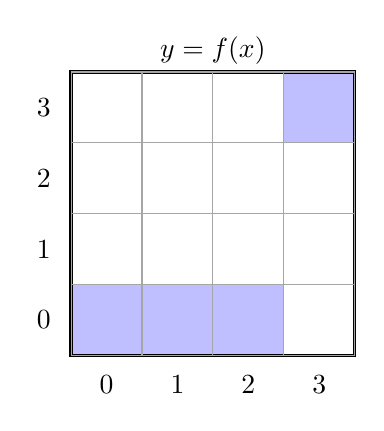
\begin{tikzpicture}[scale=0.9]
  \foreach \x/\y in {0/0,1/0,2/0,3/3} {
    \fill[blue!25] (\x,\y) rectangle ++(1,1);
  }
  \draw[very thick] (0,0) rectangle (4,4);
  \draw[step=1cm,gray!70] (0,0) grid (4,4);
  \foreach \v in {0,...,3} {
  \node[below] at (\v + 0.5,-0.15) {$\v$};
  \node[left] at (-0.15,\v + 0.5) {$\v$};
}
  \node at (2,4.3) {$y = f(x)$};
\end{tikzpicture}
\end{center}

\medskip

Because the lattice only has four elements, we can witness each adjunction by shading the pairs that satisfy the defining inequalities. Blue cells highlight the points where the inequality is tight, making the graphs of \(f\), \(g\), and \(h\) easy to spot.

\paragraph{Left adjoint $g \dashv f$}
The condition \(g(y) \leq x \iff y \leq f(x)\) means both relations pick out exactly the same lattice points:

\begin{center}
\begin{minipage}{0.45\linewidth}
\centering
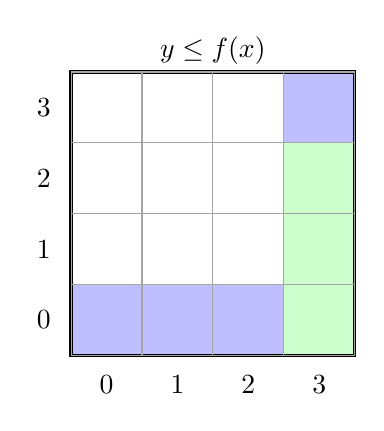
\begin{tikzpicture}[scale=0.9]
  \foreach \x in {0,...,2} {
    \fill[green!20] (\x,0) rectangle ++(1,1);
  }
  \foreach \y in {0,...,3} {
    \fill[green!20] (3,\y) rectangle ++(1,1);
  }
  \foreach \x/\y in {0/0,1/0,2/0,3/3} {
    \fill[blue!25] (\x,\y) rectangle ++(1,1);
  }
  \draw[very thick] (0,0) rectangle (4,4);
  \draw[step=1cm,gray!70] (0,0) grid (4,4);
  \foreach \v in {0,...,3} {
    \node[below] at (\v + 0.5,-0.15) {$\v$};
    \node[left] at (-0.15,\v + 0.5) {$\v$};
  }
  \node at (2,4.3) {$y \leq f(x)$};
\end{tikzpicture}
\end{minipage}\hfill
\begin{minipage}{0.45\linewidth}
\centering
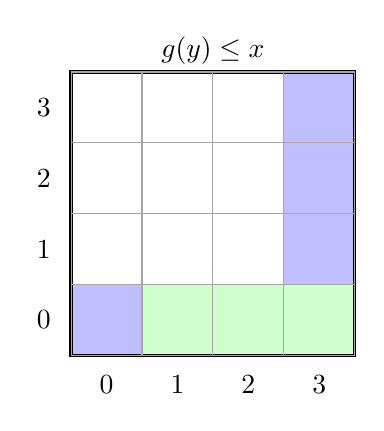
\begin{tikzpicture}[scale=0.9]
  \foreach \x in {0,...,3} {
    \fill[green!20] (\x,0) rectangle ++(1,1);
  }
  \foreach \y in {1,...,3} {
    \fill[green!20] (3,\y) rectangle ++(1,1);
  }
  \foreach \x/\y in {0/0,3/1,3/2,3/3} {
    \fill[blue!25] (\x,\y) rectangle ++(1,1);
  }
  \draw[very thick] (0,0) rectangle (4,4);
  \draw[step=1cm,gray!70] (0,0) grid (4,4);
  \foreach \v in {0,...,3} {
    \node[below] at (\v + 0.5,-0.15) {$\v$};
    \node[left] at (-0.15,\v + 0.5) {$\v$};
  }
  \node at (2,4.3) {$g(y) \leq x$};
\end{tikzpicture}
\end{minipage}
\end{center}

\smallskip
\noindent\emph{Slogan: the points below \(f\) (left) are exactly the points to the right of \(g\) (right).}

\medskip

\paragraph{Right adjoint $f \dashv h$}
Likewise, the right adjoint \(h\) is characterised by \(f(x) \leq y \iff x \leq h(y)\):

\begin{center}
\begin{minipage}{0.45\linewidth}
\centering
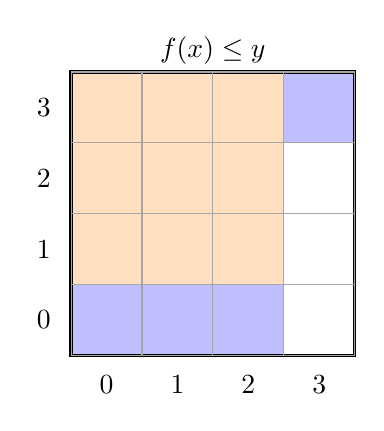
\begin{tikzpicture}[scale=0.9]
  \foreach \x in {0,...,2} {
    \foreach \y in {0,...,3} {
      \fill[orange!25] (\x,\y) rectangle ++(1,1);
    }
  }
  \fill[orange!25] (3,3) rectangle ++(1,1);
  \foreach \x/\y in {0/0,1/0,2/0,3/3} {
    \fill[blue!25] (\x,\y) rectangle ++(1,1);
  }
  \draw[very thick] (0,0) rectangle (4,4);
  \draw[step=1cm,gray!70] (0,0) grid (4,4);
  \foreach \v in {0,...,3} {
    \node[below] at (\v + 0.5,-0.15) {$\v$};
    \node[left] at (-0.15,\v + 0.5) {$\v$};
  }
  \node at (2,4.3) {$f(x) \leq y$};
\end{tikzpicture}
\end{minipage}\hfill
\begin{minipage}{0.45\linewidth}
\centering
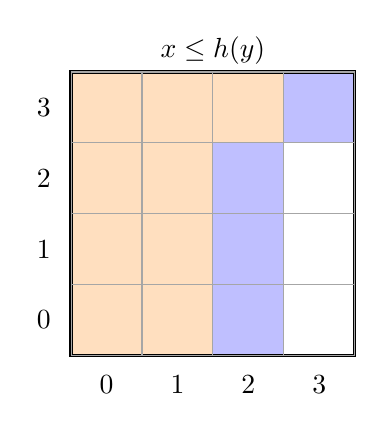
\begin{tikzpicture}[scale=0.9]
  \foreach \y in {0,...,2} {
    \foreach \x in {0,...,2} {
      \fill[orange!25] (\x,\y) rectangle ++(1,1);
    }
  }
  \foreach \x in {0,...,3} {
    \fill[orange!25] (\x,3) rectangle ++(1,1);
  }
  \foreach \x/\y in {2/0,2/1,2/2,3/3} {
    \fill[blue!25] (\x,\y) rectangle ++(1,1);
  }
  \draw[very thick] (0,0) rectangle (4,4);
  \draw[step=1cm,gray!70] (0,0) grid (4,4);
  \foreach \v in {0,...,3} {
    \node[below] at (\v + 0.5,-0.15) {$\v$};
    \node[left] at (-0.15,\v + 0.5) {$\v$};
  }
  \node at (2,4.3) {$x \leq h(y)$};
\end{tikzpicture}
\end{minipage}
\end{center}

\smallskip
\noindent\emph{Slogan: the points above \(f\) (left) are exactly the points to the left of \(h\) (right).}

\end{document}
